\documentclass[12pt, twoside]{article}
\usepackage[utf8]{inputenc}
\usepackage[english,russian]{babel}
\newcommand{\hdir}{.}

\usepackage{graphicx}
\usepackage{caption}
\usepackage{amssymb}
\usepackage{amsmath}
\usepackage{mathrsfs}
\usepackage{euscript}
\usepackage{upgreek}
\usepackage{array}
\usepackage{theorem}
\usepackage{graphicx}
\usepackage{subfig}
\usepackage{caption}
\usepackage{color}
\usepackage{url}

\usepackage[left=2cm,right=2cm,top=3cm,bottom=2cm,bindingoffset=0cm]{geometry}

\usepackage{fancyhdr}
\pagestyle{fancy}
\fancyhead{}
\fancyhead[LE,RO]{\thepage} 
\fancyhead[CO,CE]{Лекция 2}
\fancyhead[LO,LE]{Грабовой Андрей}

\begin{document} 

\begin{center}
{\LARGE\bf
Основные понятия в машинном обучении
}
\end{center}

Данная лекция сделана на основе лекций Воронцова Константина Вячеславовича, которые он читает на кафедре <<Интеллектуальные системы>> ФУПМ МФТИ. 

\section{Постановка задачи}

\subsection{Что задано?}
\begin{itemize}
	\item задано множество объектов $\textbf{X}$,
	\item задано множество ответов $\textbf{Y}$,
	\item задана некоторая неизвестная функция $\textbf{f}: \textbf{X} \rightarrow \textbf{Y}$.
\end{itemize}

Очевидно, что мы не знаем истиной $\textbf{f}$. Тогда давайте будем играть в следующую игру, нам дают некоторые $x \in \textbf{X}$ и дают ответ $y = \textbf{f}(x)$, а мы хотим найти истинное $\textbf{f}$.

\subsection{Формальная постановка задачи}
\begin{itemize}
	\item дано множество объектов $\{x_1, \cdots x_l\} \subset \textbf{X}$,
	\item дано множество ответов $y_i = \textbf{f}(x_i), i=1,\cdots, l$,
	\item найти алгоритм $\textbf{a}:\textbf{X} \rightarrow \textbf{Y}$ --- приближающий неизвестную функцию $\textbf{f}$.
\end{itemize}

Под $\textbf{a}:\textbf{X} \rightarrow \textbf{Y}$ понимается некоторая функция, которая каждому объекту из множества $\textbf{X}$ ставит в соответствие некоторый элемент из \textbf{Y}.

\subsection{В чем задача машинного обучения?}
\begin{itemize}
	\item понять как задаются объекты и какими могут быть ответы
	\item ответить на вопрос в каком смысле $\textbf{a}$ приближает $\textbf{f}$
	\item понять как строить отображение $\textbf{a}$
\end{itemize}

На эти $3$ вопроса мы и будем пытаться отвечать в течении нашего курса.

\section{Задание объектов}
	
	Каждый объект выборки задается некоторым набором признаков (features). Что такое признаки? Признаком может быть все что угодно. Например если объект это человек, то в качестве признаков может быть рост, цвет глаз, вес, цвет волос, пол человека и т.д.

\subsection{Как задать описание объктов?}
$$f_{j}:X \rightarrow D_j,\quad j = 1,\cdots, n, \eqno(1)$$
где $n$ это количество признаков для каждого элемента в нашей выборке.

Что такое $f_j$? $f_j$ это такая функция над объектом $x$, которая возвращает $j$-й признак объекта. Например у нас  выборка $\textbf{X}$ это люди, тогда $f_j$ это например функция которая по заданному человеку $x$ возвращает его вес.

Тогда рассмотрим матрицу <<объект---признак>>:

$$\textbf{F} = ||f_j(x_i)||_{l\times n} = 
\begin{bmatrix}
f_1(x_1) &\cdots & f_n(x_1)\\
\cdots & \cdots & \cdots\\
 f_1(x_l) &\cdots & f_n(x_l)\\
\end{bmatrix}.
\eqno(2)
$$

 Тоесть матрица $\textbf{F}$ это матрица которая имеет количество строк равное количеству объектов, а количество столбцов равно количеству признаков.
 
 В нас в курсе у нас всегда изначально будет задана матрица $\textbf{F}$. Но в общем случаи придумать признаковое описание объектов является достаточно трудной задачей.
 
 \section{Задание ответов}
 \paragraph{Классификация}:
 \begin{itemize}
 	\item $\textbf{Y} = \{0, 1\}$ --- классификация на $2$ класса (если в примере с людьми то м. или ж.),
	\item $\textbf{Y} = \{0, 1, \cdots, M\}$ --- классификация на $M$ классов (к пример с людьми это цвет волос).
 \end{itemize}
 
 \paragraph{Регрессия}:
 \begin{itemize}
 	\item $\textbf{Y} = \mathbb{R}^n$ --- в качестве ответом у нас может быть вся числовая ось при $n=1$.
 \end{itemize}
 
 \section{Примеры смысла <<$\textbf{a}$ приближает $\textbf{f}$>>}
 
 \begin{center}
Задача {\bf регрессии}.
 \end{center}
 
 Пусть у нас есть множество истинных ответов $\{\textbf{y}_1,\cdots, \textbf{y}_l\}$ и множество ответов которые нам дает алгоритм $\textbf{a}$.
 
 Определим $\delta(\textbf{a})$ --- как ошибку которую допускает алгоритм $\textbf{a}$ на данном нам множестве $\{x_1, \cdots x_l\} \subset \textbf{X}$.
 
 $$\delta{\textbf{a}} = \sum_{k=1}^{l}||\textbf{a}(x_k) - y_k||^2, \eqno(3)$$
 где под $||\textbf{a}(x_k) - y_k||$ --- подразумевается расстояние от предсказанного ответа до истинного. К примеру, если $Y=\mathbb{R}$, то в качестве расстояния можно взять модуль разности чисел.
 
  \begin{center}
Задача {\bf классификации}.
 \end{center}

 Определим $\delta(\textbf{a})$ --- как ошибку которую допускает алгоритм $\textbf{a}$ на данном нам множестве $\{x_1, \cdots x_l\} \subset \textbf{X}$.

$$\delta{\textbf{a}} = \sum_{k=1}^{l}[\textbf{a}(x_k) \not= y_k], \eqno(4)$$
где $[\textbf{a}(x_k) \not= y_k]$ это 1, если условие в скобках истинное и 0 если ложное. Простыми словами $\delta{\textbf{a}}$  определили как количество ошибок в классификации. 

 \section{Примеры задач}
 \begin{center}
Задача {\bf регрессии}.
 \end{center}

Рассмотрим постановочную задачу регрессии.
\subsection{Что дано?}
\begin{itemize}
	\item $\textbf{X} = \mathbb{R}$ --- множество объектов,
	\item $\textbf{Y} = \mathbb{R}$ --- множество ответов,
	\item неизвестная функция \textbf{f} пусть будет просто квадратичная, то есть $y = \textbf{f}(x) = x^2$ 
\end{itemize}

\subsection{По каким данным мы восстанавливаем неизвестную функцию?}
\begin{figure}[h!t]\center
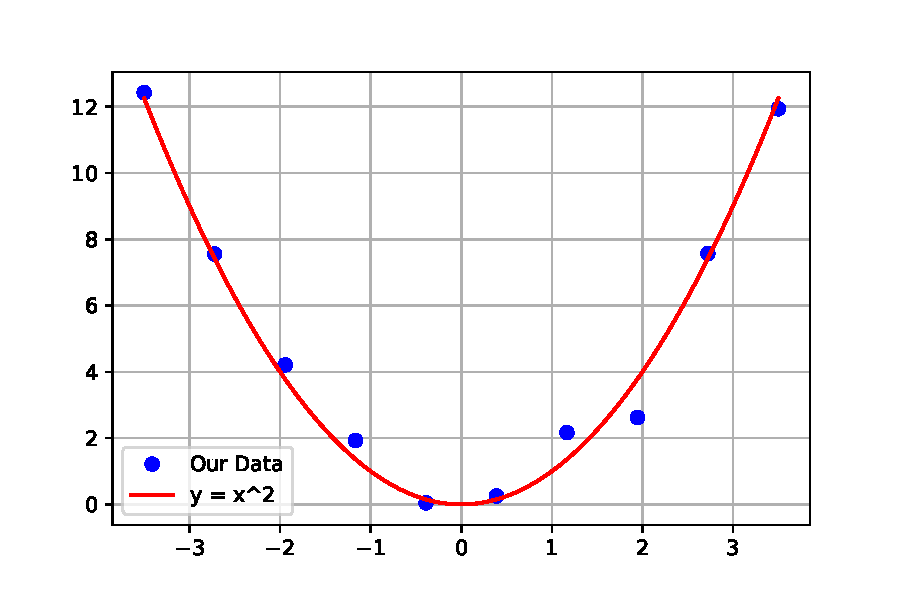
\includegraphics[width=0.7\textwidth]{Lecture_2_regress.pdf}
\caption{Данные данные для нахождения $\textbf{a}$}
\label{Lecture_2_regress}
\end{figure}

На рис.~\ref{Lecture_2_regress} показаны данные по которым мы должно построить отображение $\textbf{a}$. По оси абсцисс отложены значения $\{x_1, \cdots, x_{10}\} \subset X$, а по оси ординат отложены значения $\{y_1, \cdots, y_{10}\} \subset Y$. Также на графике построен график функции $y = x^2$. Как видно из графика синие точке не ложатся идеально на красный график. Это все из-за того, что данные не бывают идеальные, об этом мы поговорим чуть позже.

  \begin{center}
Задача {\bf классификации}.
 \end{center}
 
 Рассмотрим постановочную задачу классификации.
\subsection{Что дано?}
\begin{itemize}
	\item $\textbf{X} = \mathbb{R}^2$ --- множество объектов,
	\item $\textbf{Y} = \{0,1\}$ --- множество ответов,
	\item неизвестная функция \textbf{f} 
\end{itemize}

\subsection{По каким данным мы восстанавливаем неизвестную функцию?}
\begin{figure}[h!t]\center
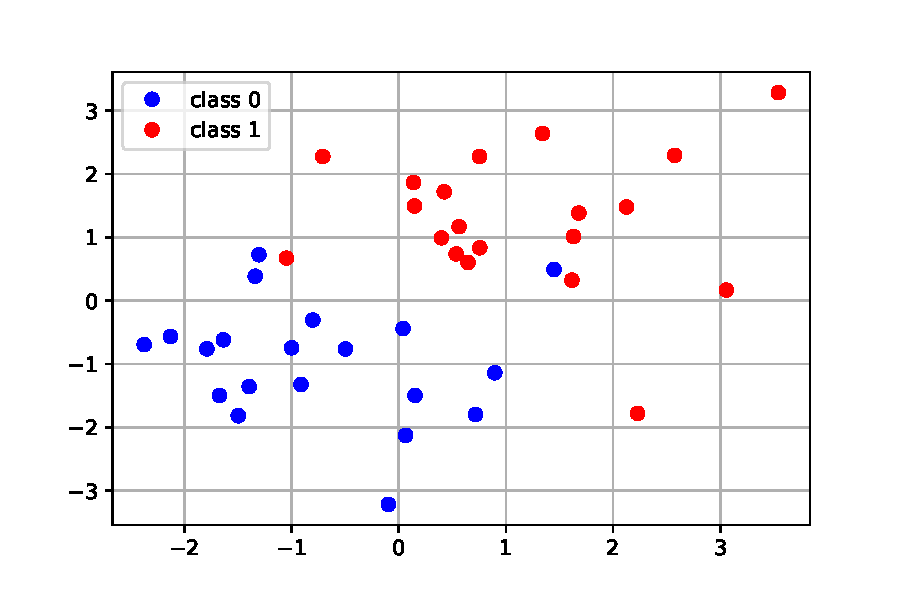
\includegraphics[width=0.7\textwidth]{Lecture_2_class.pdf}
\caption{Данные данные для нахождения $\textbf{a}$}
\label{Lecture_2_class}
\end{figure}

\section{Метод k - ближайших соседей}
 \begin{center}
Задача {\bf классификации}.
 \end{center}

Данный метод является очень простым. Пусть мы можем измерить расстояние между любыми объектами из множества $\textbf{X}$. Тогда алгоритм заключается в том, чтобы найти тот класс которого больше всего среди $k-$ближайших соседей.

\subsection{Алгоритм}

$\text{k} = 9$ --- сколько соседей будем учитывать\\
$\text{M} = 2$ --- количество классов\\
$\{x_1, \cdots, x_l\}$ --- объекты для которых мы знаем ответы\\
$\{y_1, \cdots, y_l\}$ --- ответы\\
$\text{x}$ --- нужно класифицировать\\
$\text{mesure}$ ---  строим массив расстояний от x до каждого $x_i$\\
$\text{mesure} = \text{mesure}.\text{sort}$ ---  сортируем его по возрастанию (паралельно нужно сортировать и $\text{y}$)\\
$\text{arr}$ --- массив счетчик каждого класса среди $k$ ближайших\\
$\text{for}~i~\text{in}~\text{k}$\\
$....\text{arr}[y_i] = \text{arr}[y_i]  + 1$ 



\begin{thebibliography}{99}
	\bibitem{vokov}
	\textit{Воронцов К. В.} Машинное обучение // Годовой курс кафедры <<Интеллектуальные системы>> Москва, 2018.
	\url{http://www.machinelearning.ru/wiki/index.php?title=Vokov}
\end{thebibliography}



\end{document} 